\documentclass[12pt]{article}
\usepackage{geometry}
\geometry{a4paper, margin=1in}
\usepackage{amsmath}   % For mathematical symbols and equations
\usepackage{graphicx}  % For including images
\usepackage{hyperref}  % For hyperlinks
\usepackage{siunitx}
\usepackage{float}
\usepackage{verbatim}

% Title Page
\title{PHYS 2801 - Assignment 2}
\author{Son Thanh Truong}
\date{\today}  % Current date


\begin{document}

\maketitle

% Main section header
\section{Question 1: The Maxwell–Boltzmann distribution}

The Maxwell–Boltzmann distribution:

% Can use a subsection for each question
\subsection{Part (a)}
Here is the Maxwell–Boltzmann distribution function:
\begin{equation}
 % f(v) = 4 \pi \left( \frac{m}{2 \pi k_B T} \right)^{3/2} v^2 \exp\left( -\frac{m v^2}{2 k_B T} \right)
  f(v) = 4 \pi \left( \frac{m}{2 \pi k_B T} \right)^{3/2} v^2 \exp\left( -\frac{m v^2}{2 k_B T} \right)
  \label{eq:maxwell-speed}
\end{equation}
% We can now refer to the equation using the label
The Maxwell-Boltzmann distribution tells us what fraction of the particles 
are moving slow or fast. 
If integrated over all speeds from 0 to infinity, the result is 1.
f is the probability density, v is the particle speeds, m is the mass of the particles, T is the temperature, and kB is the Boltzmann constant.

\begin{figure}[H]
    \centering
    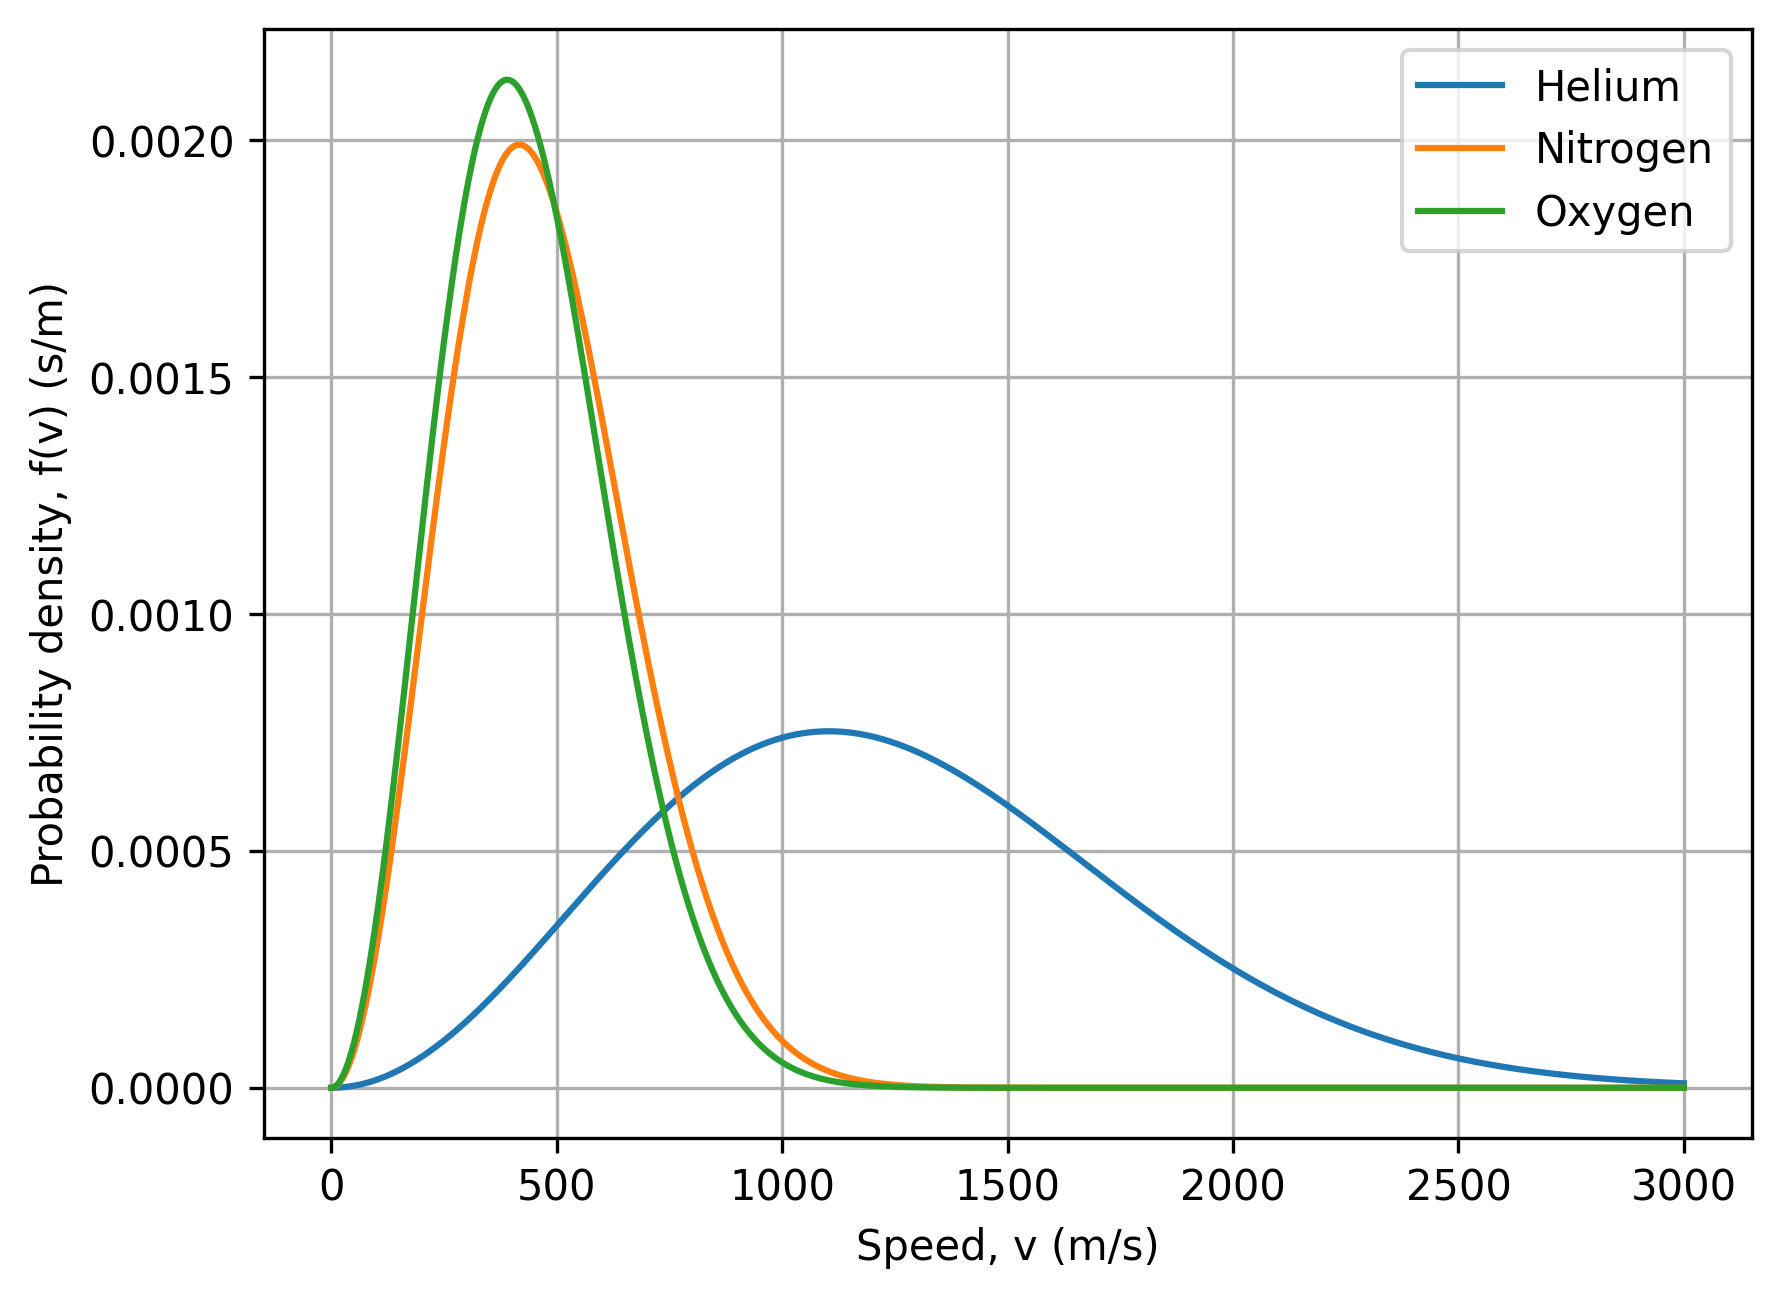
\includegraphics[width=0.8\textwidth]{maxwell_boltzmann.png}
    \caption{The Maxwell-Boltzmann distribution of particle speeds at temperature T=293.15K.
    Notice how Helium, because of being lighter has a distribution shifted more to the right 
    meaning a bigger percentage of the helium has faster speeds compared to the other two 
    elements. This plot was made using the equation as given in Eq.~\ref{eq:maxwell-speed}}
    \label{fig:maxwell-boltzmann}
\end{figure}

\verbatiminput{mystery_program.txt}
\verbatiminput{mystery.txt}

c) cxx files are instructions for a computer on a higher end, meaning it is more readable
like a human language. exe files are more low end meaning it is closer to how computers talk.
Because of this, lower end exe files run much faster than the higher end counterparts because
higher level languages have to be translated to machine code before running.

d) Based on the text output file I'd say the programmer was Indian, because the image looks like
the map of India.

\end{document}

